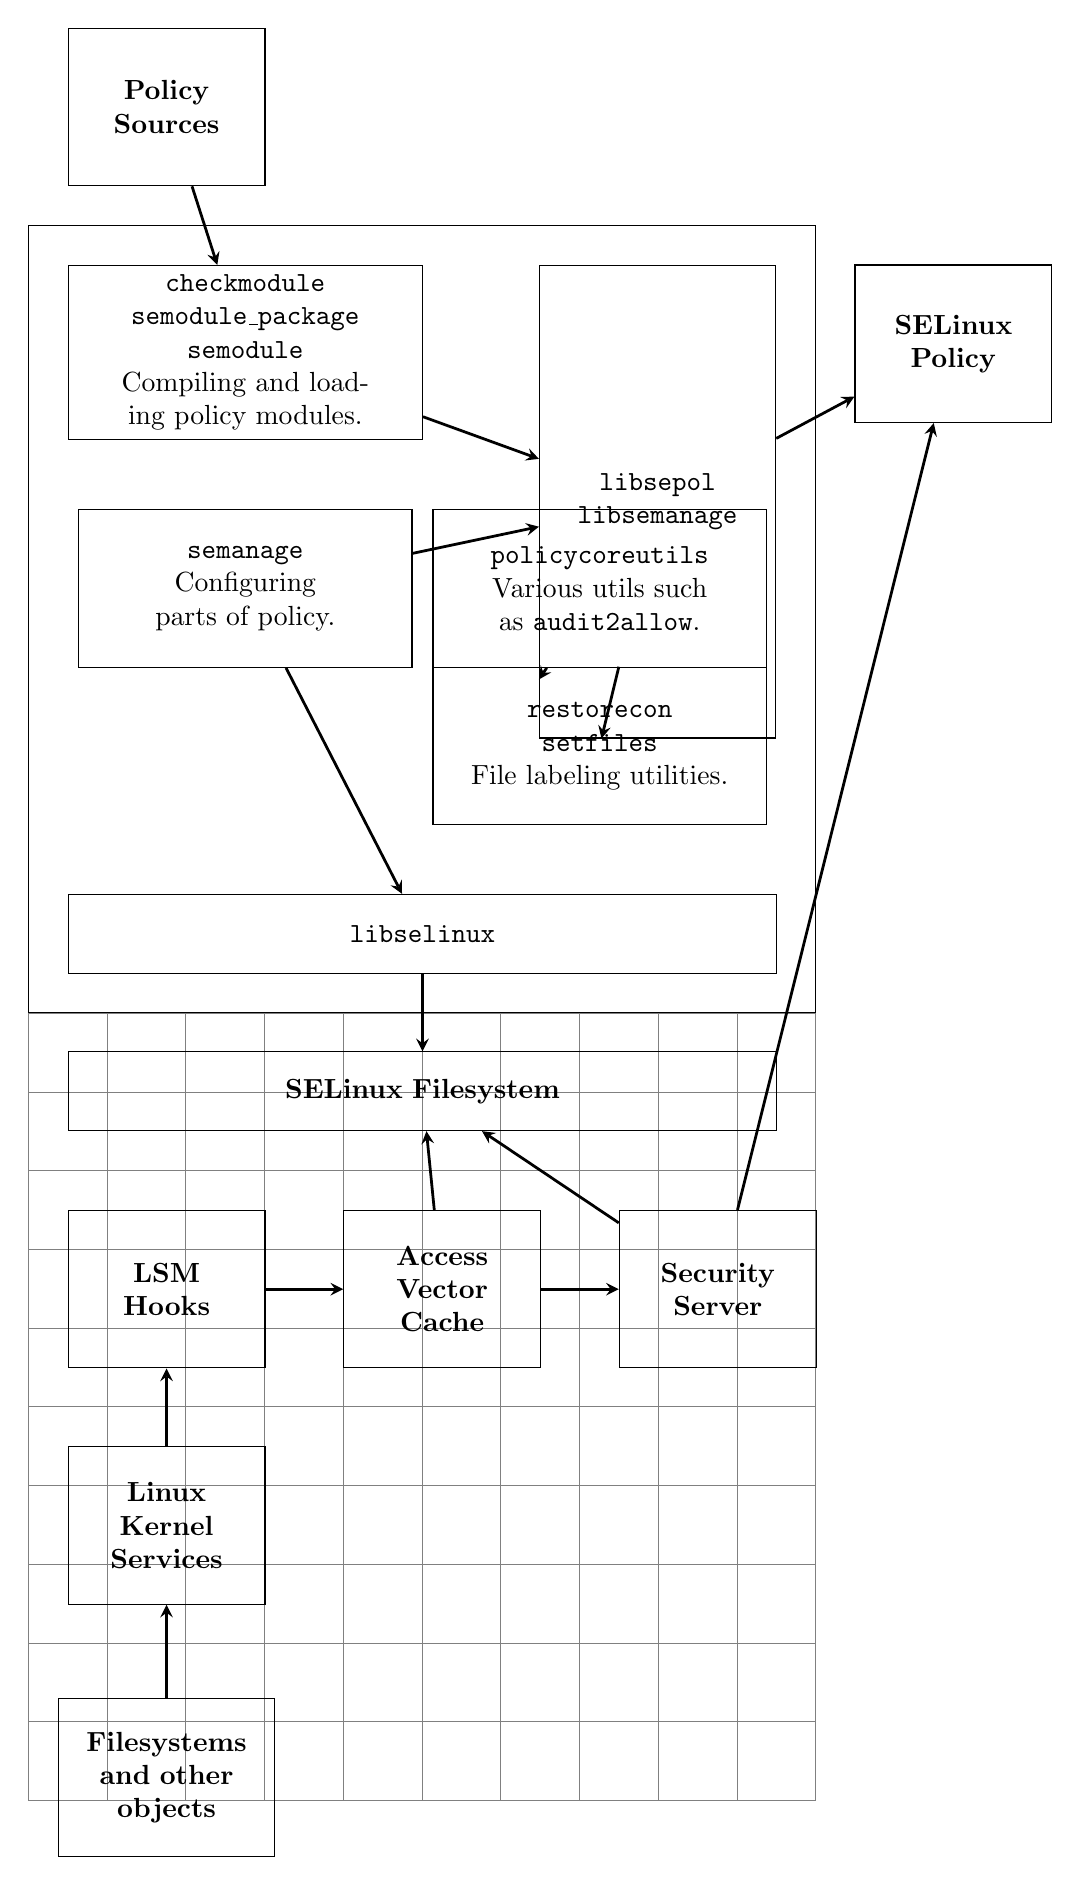
\begin{tikzpicture}
    \usetikzlibrary{calc}
    \tikzstyle{line} = [->,>=stealth, line width=1pt]
    \tikzstyle{rec} = [rectangle, draw=black, align=center, text width=4cm,
        minimum height=2cm, minimum width=2cm]

    \draw (0,0) rectangle (10,-10);
    \draw[step=1cm,gray,very thin] (0,-20) grid (10,-10);

    \node(policysource) [rec, text width=2cm, minimum width=2.5cm]
        at (0.5,0.5) [anchor=south west]
        {\textbf{Policy Sources}};
    \node(compiling) [rec, text width=4cm, minimum width=4.5cm]
        at (0.5,-0.5) [anchor=north west]
        {\textbf{\texttt{checkmodule}\\ \texttt{semodule\_package}\\
        \texttt{semodule}}\\ Compiling and loading policy modules.};
    \node(libsepol) [rec, text width=2.5cm, minimum width=3cm, minimum
        height=6cm]
        at (9.5,-0.5) [anchor=north east]
        {\textbf{\texttt{libsepol}\\ \texttt{libsemanage}}};
    \node(policy) [rec, text width=2cm, minimum width=2.5cm]
        at (11.75,-1.5)
        {\textbf{SELinux Policy}};
    \node(semanage) [rec, below of=compiling, node distance=3cm]
        {\textbf{\texttt{semanage}}\\ Configuring parts of policy.};
    \node(policycoreutils) [rec, right of=semanage, node distance=4.5cm]
        {\textbf{\texttt{policycoreutils}}\\ Various utils such as
        \texttt{audit2allow}.};
    \node(restorecon) [rec, below of=policycoreutils, node distance=2cm]
        {\textbf{\texttt{restorecon}\\ \texttt{setfiles}}\\ File labeling
        utilities.};
    \node(libselinux) [rec, text width=8.5cm, minimum width=9cm, minimum
        height=1cm]
        at (0.5,-9.5) [anchor=south west]
        {\textbf{\texttt{libselinux}}};
    \node(selinuxfs) [rec, text width=8.5cm, minimum width=9cm, minimum
        height=1cm, below of=libselinux, node distance=2cm]
        {\textbf{SELinux Filesystem}};
    \node(kernelservices) [rec, text width=2cm, minimum width=2.5cm]
        at (0.5,-15.5) [anchor=north west]
        {\textbf{Linux Kernel Services}};
    \node(fs) [rec, text width=2.5cm, below of=kernelservices,
        node distance=3.2cm] {\textbf{Filesystems and other objects}};
    \node(lsmhooks) [rec, text width=2cm, minimum width=2.5cm]
        at (0.5,-12.5) [anchor=north west]
        {\textbf{LSM Hooks}};
    \node(avc) [rec, text width=2cm, minimum width=2.5cm, right of=lsmhooks,
        node distance=3.5cm]
        {\textbf{Access Vector Cache}};
    \node(secser) [rec, text width=2cm, minimum width=2.5cm, right of=avc,
        node distance=3.5cm]
        {\textbf{Security Server}};

    \draw[line] (policysource) -- (compiling);
    \draw[line] (compiling) -- (libsepol);
    \draw[line] (libsepol) -- (policy);
    \draw[line] (semanage) -- (libsepol);
    \draw[line] (semanage) -- (libselinux);
    \draw[line] (libselinux) -- (selinuxfs);
    \draw[line] (policycoreutils) -- (libsepol);
    \draw[line] (restorecon) -- (libsepol);
    \draw[line] (fs) -- (kernelservices);
    \draw[line] (kernelservices) -- (lsmhooks);
    \draw[line] (lsmhooks) -- (avc);
    \draw[line] (avc) -- (secser);
    \draw[line] (avc) -- (selinuxfs);
    \draw[line] (secser) -- (policy);
    \draw[line] (secser) -- (selinuxfs);

    %\draw[line] () -- ();
\end{tikzpicture}
